\section{Philosophy}

\begin{frame}{Why Rasterization?}
  \pause
  \begin{minipage}{0.45\textwidth}
    \centering
    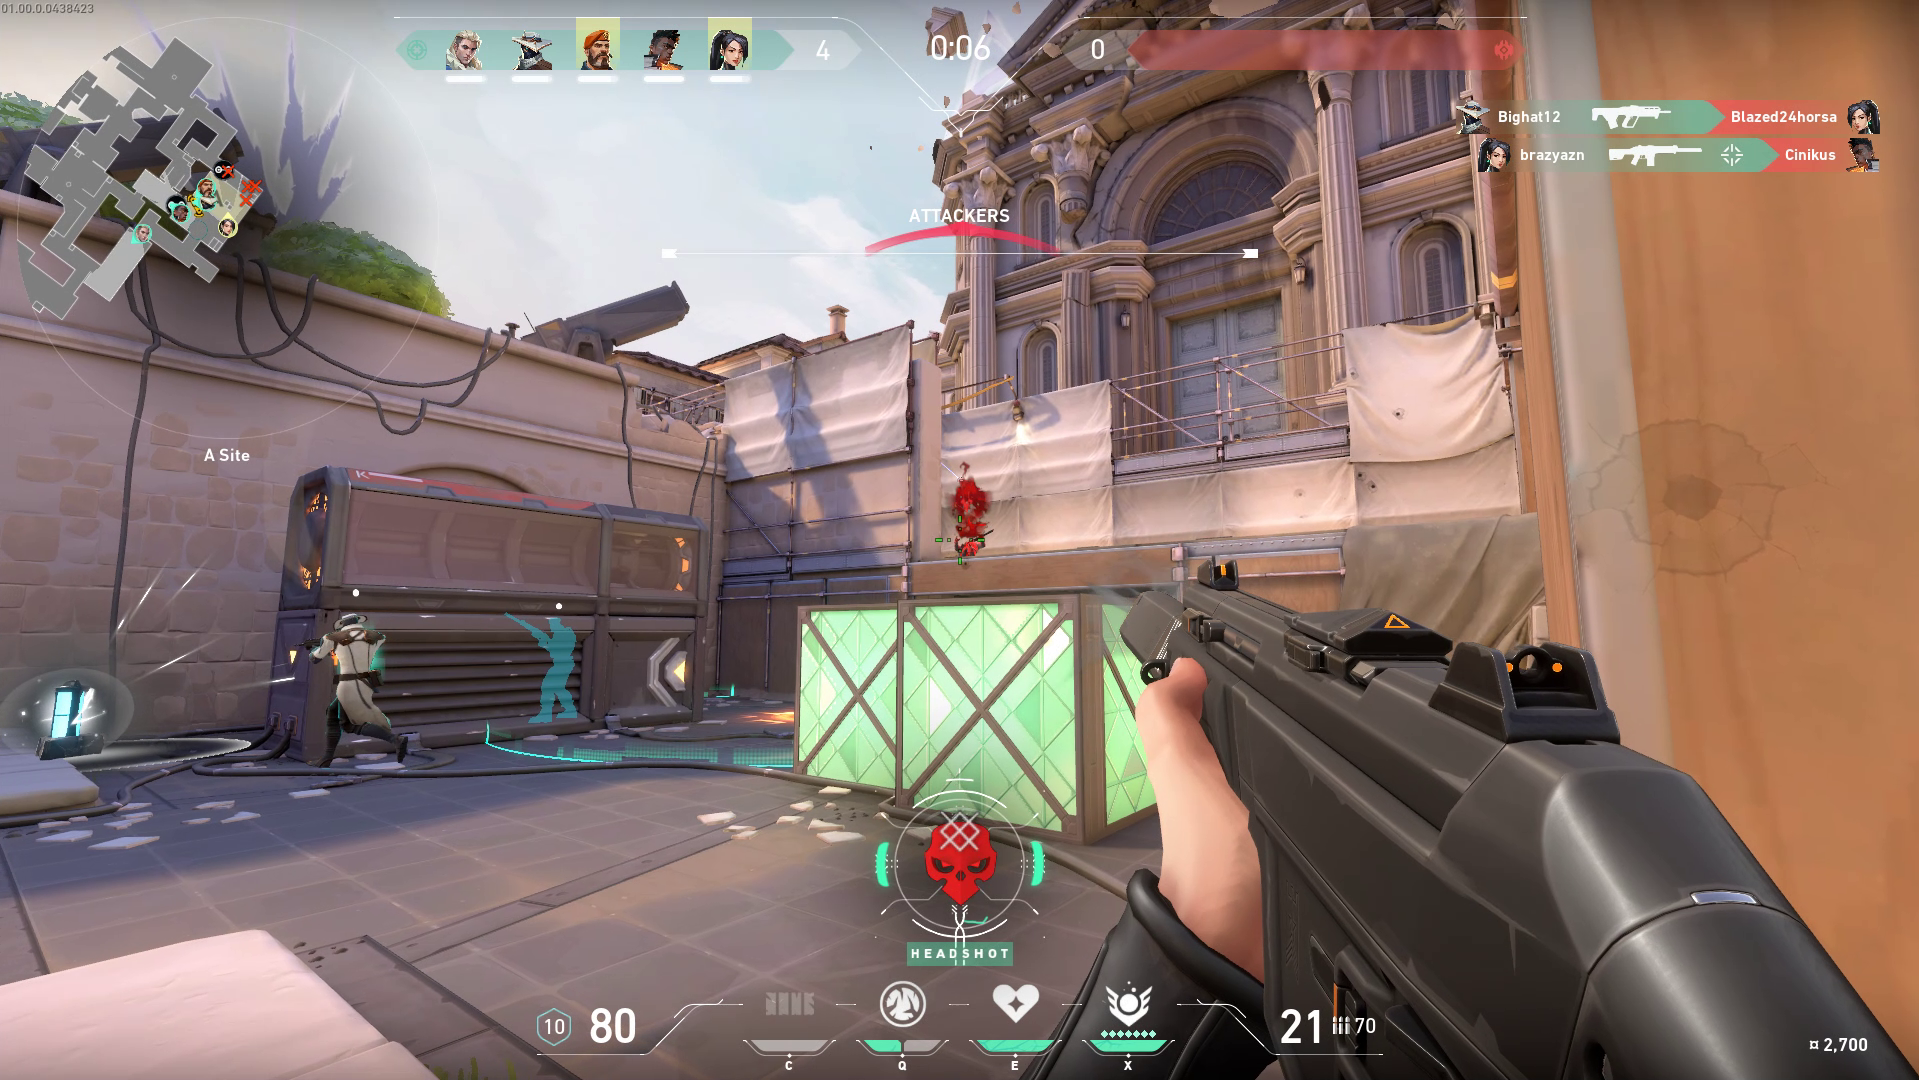
\includegraphics[width=\linewidth]{images/valorant_gameplay.png}
    \captionof*{figure}{Valorant - 120 FPS Gaming}
  \end{minipage}%
  \hfill
  \pause
  \begin{minipage}{0.45\textwidth}
    \centering
    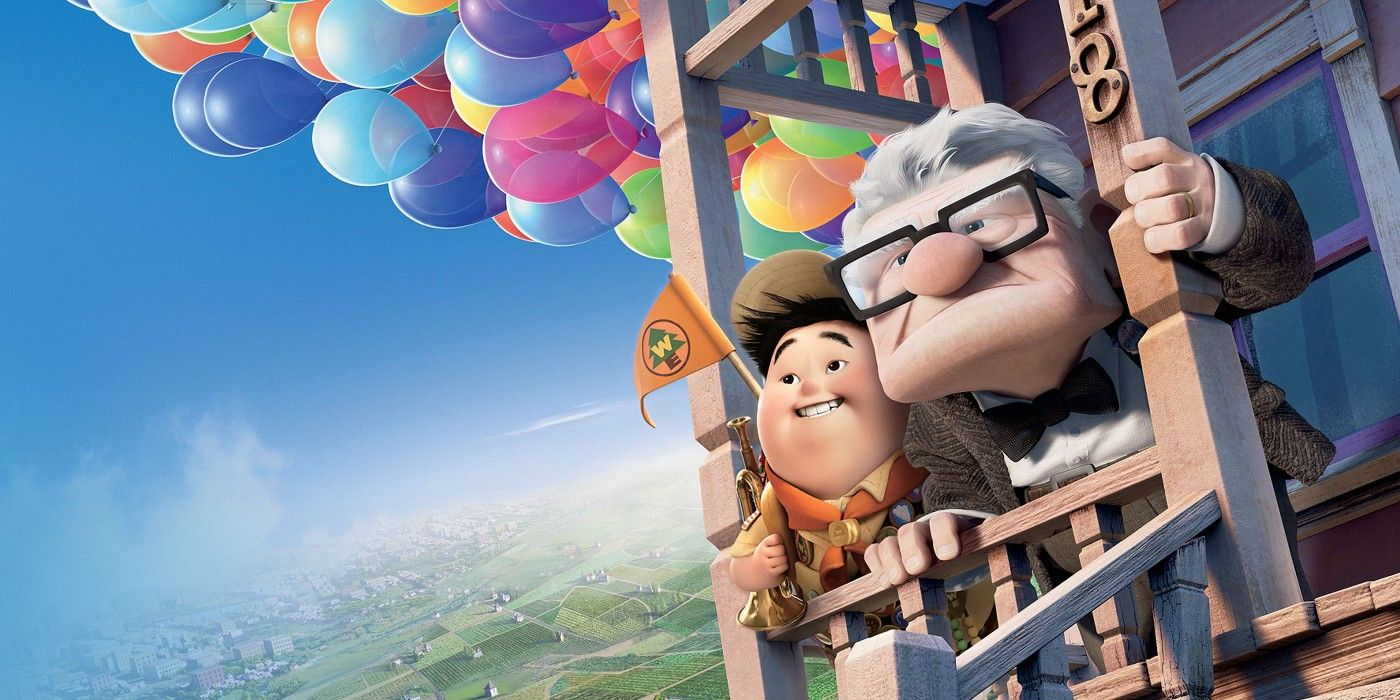
\includegraphics[width=\linewidth]{images/pixar_movie.jpg}
    \captionof*{figure}{Pixar Movie - 30 hours per frame}
  \end{minipage}

  \begin{itemize}
    \item<3-> \textbf{Real-time constraint:} Games need 60-120 FPS
    \item<4-> \textbf{Interactive experience:} User input must feel responsive
    \item<5-> \textbf{Trade-off:} Sacrifice physical accuracy for speed
    \item<6-> \textbf{Goal:} Images that look good enough, delivered fast enough
  \end{itemize}
\end{frame}

\section{The Speed vs Accuracy Trade-off}

\begin{frame}{Rasterization vs Ray Tracing: The Fundamental Choice}
  \begin{center}
    \begin{tikzpicture}[scale=0.9]
      % Rasterization side
      \node[rectangle, draw, minimum width=3cm, minimum height=2cm, fill=PrimaryColor!20] (raster) at (0,0) {\faIcon{tachometer-alt} Rasterization};
      \node[above] at (0,1.5) {\textbf{Fast Approximations}};

      % Ray tracing side
      \node[rectangle, draw, minimum width=3cm, minimum height=2cm, fill=AccentColor!20] (ray) at (6,0) {\faIcon{eye} Ray Tracing};
      \node[above] at (6,1.5) {\textbf{Physical Accuracy}};

      % Trade-off arrow
      \draw[<->, very thick, SecondaryColor]
      (raster.east) -- (ray.west)
      node[midway, above, text=SecondaryColor, font=\footnotesize]{Trade-off};

      % Characteristics
      \node[below] at (0,-2.5) {
        \begin{minipage}{4cm}
          \textcolor{PrimaryColor}{\textbf{Rasterization:}}
          \begin{itemize}
              \scriptsize
            \item 60-240 FPS
            \item Clever approximations
            \item Hardware optimized
            \item "Good enough" quality
          \end{itemize}
        \end{minipage}
      };

      \node[below] at (6,-2.5) {
        \begin{minipage}{4cm}
          \textcolor{AccentColor}{\textbf{Ray Tracing:}}
          \begin{itemize}
              \scriptsize
            \item 0.1-30 FPS
            \item Physical simulation
            \item Computationally heavy
            \item Photorealistic
          \end{itemize}
        \end{minipage}
      };
    \end{tikzpicture}
  \end{center}
\end{frame}

\begin{frame}{The Real-Time Graphics Challenge}
  \begin{columns}
    \begin{column}{0.6\textwidth}
      \begin{conceptbox}{Time Budget at 60 FPS}
        \begin{center}
          \large $\frac{1}{60} = 16.67$ milliseconds per frame
        \end{center}

        \vspace{0.3cm}
        \textbf{What needs to happen:}
        \begin{itemize}
          \item Process input
          \item Update game logic
          \item Render graphics
          \item Present to screen
        \end{itemize}

        \vspace{0.3cm}
        \textbf{Graphics budget:} $\sim$10-12ms
      \end{conceptbox}
    \end{column}
    \begin{column}{0.4\textwidth}
      \begin{tikzpicture}[scale=0.8]
        % Timeline
        \draw[thick, PrimaryColor] (0,0) -- (0,6);
        \node[left] at (1.6,6.7) {\textbf{16.67ms}};

        % Segments
        \fill[SecondaryColor!30] (0,0) rectangle (1,1);
        \node[right] at (1.1,0.5) {\scriptsize Input (1ms)};

        \fill[AccentColor!30] (0,1) rectangle (1,2.5);
        \node[right] at (1.1,1.75) {\scriptsize Game Logic (1.5ms)};

        \fill[PrimaryColor!30] (0,2.5) rectangle (1,5.5);
        \node[right] at (1.1,4) {\scriptsize \textbf{Graphics (12ms)}};

        \fill[LightGray] (0,5.5) rectangle (1,6);
        \node[right] at (1.1,5.75) {\scriptsize Present (0.5ms)};

      \end{tikzpicture}
    \end{column}
  \end{columns}
\end{frame}

\begin{frame}{How Rasterization Achieves Speed}
  \begin{center}
    \begin{tikzpicture}[scale=1]
      % Central concept
      \node[circle, draw, fill=PrimaryColor!20, minimum size=2cm] (center) at (0,0) {
        \begin{minipage}{1.5cm}
          \centering
          \textbf{Smart} \\
          \textbf{Approx.}
        \end{minipage}
      };

      % Surrounding strategies
      \node[rectangle, draw, fill=SecondaryColor!20, text width=2cm, text centered] (parallel) at (3,2) {
        Massive \\
        Parallelism
      };

      \node[rectangle, draw, fill=AccentColor!20, text width=2cm, text centered] (hardware) at (3,-2) {
        Dedicated \\
        Hardware
      };

      \node[rectangle, draw, fill=ObjectColor!20, text width=2cm, text centered] (approx) at (-3,2) {
        Local \\
        Lighting
      };

      \node[rectangle, draw, fill=LightColor!20, text width=2cm, text centered] (cached) at (-3,-2) {
        Precomputed \\
        Data
      };

      % Connections
      \draw[->, thick] (center) -- (parallel);
      \draw[->, thick] (center) -- (hardware);
      \draw[->, thick] (center) -- (approx);
      \draw[->, thick] (center) -- (cached);

      % Examples
      \node[below, text width=2.5cm, text centered] at (parallel.south) {
        \scriptsize Process thousands of triangles simultaneously
      };

      \node[above, text width=2.5cm, text centered] at (hardware.north) {
        \scriptsize Fixed-function rasterizers, Z-buffers
      };

      \node[below, text width=2.5cm, text centered] at (approx.south) {
        \scriptsize Ignore global illumination, use simple models
      };

      \node[above, text width=2.5cm, text centered] at (cached.north) {
        \scriptsize Shadow maps, light maps, textures
      };
    \end{tikzpicture}
  \end{center}
\end{frame}

\begin{frame}{The Clever Approximations}
  \begin{columns}
    \begin{column}{0.5\textwidth}
      \begin{raybox}{What We Skip}
        \begin{itemize}
          \item \textbf{Global illumination:} No light bouncing
          \item \textbf{Perfect shadows:} Use shadow maps
          \item \textbf{Perfect reflections:} Use environment maps
          \item \textbf{Complex materials:} Simplified BRDFs
        \end{itemize}
      \end{raybox}
    \end{column}
    \begin{column}{0.5\textwidth}
      \begin{conceptbox}{What We Gain}
        \begin{itemize}
          \item \textbf{Predictable performance:} Linear with triangle count
          \item \textbf{Hardware optimization:} Purpose-built silicon
          \item \textbf{Real-time interaction:} Immediate feedback
          \item \textbf{Scalable quality:} Adjust for performance
        \end{itemize}
      \end{conceptbox}
    \end{column}
  \end{columns}

\end{frame}
